\documentclass[final]{article}

\usepackage{aps360}
\usepackage[utf8]{inputenc}
\usepackage[T1]{fontenc}
\usepackage{hyperref}
\usepackage{url}
\usepackage{booktabs}
\usepackage{amsmath}
\usepackage{amssymb}
\usepackage{microtype}
\usepackage{graphicx}
\graphicspath{{image/}}
\usepackage{tikz}
\usetikzlibrary{arrows.meta, positioning, calc}

% Reduce space between section headers and body text
\makeatletter
\renewcommand{\section}{%
  \@startsection{section}{1}{\z@}%
                {-1.5ex \@plus -0.3ex \@minus -0.2ex}%
                {0.4ex \@plus 0.1ex}%
                {\large\bf\raggedright}%
}
\makeatother

% Slightly tighten inter-paragraph spacing to keep the main text within 4 pages
\setlength{\parskip}{2.6pt}

% Override geometry: tighter top/bottom margins
\AtBeginDocument{%
  \newgeometry{%
    textheight=9.5in,
    textwidth=5.5in,
    top=0.65in,
    headheight=12pt,
    headsep=15pt,
    footskip=18pt%
  }%
}

\title{Pose-Based Human Action Recognition for Athletic Movement Analysis\\\large Final Report}
\author{%
  Harry Zhang\\
  1010988843, harryh.zhang@mail.utoronto.ca\\
  https://github.com/po8onthetrack/Deep-Learning-Project\\
}

\begin{document}

\maketitle
\vspace{-0.45in}

\section*{Introduction}
Motivated by the author's badminton and bouldering experience, this project performs markerless action recognition from pose alone: a 30-frame sequence of 17 body keypoints from a single camera (the \textbf{input}) is classified into one of 20 MPOSE2021 action categories (the \textbf{output}), a building block for movement analysis and technique feedback. Deep learning fits because an action is defined by \emph{how} joints move over time --- a spatio-temporal pattern no fixed rule can capture but a recurrent network can learn \citep{du2015hierarchical}.\footnote{Portions of the writing and code in this project were developed with the assistance of Claude \citep{anthropic2026claude} and Claude Code \citep{anthropic2026claudecode}.}

\begin{figure}[!h]
\centering
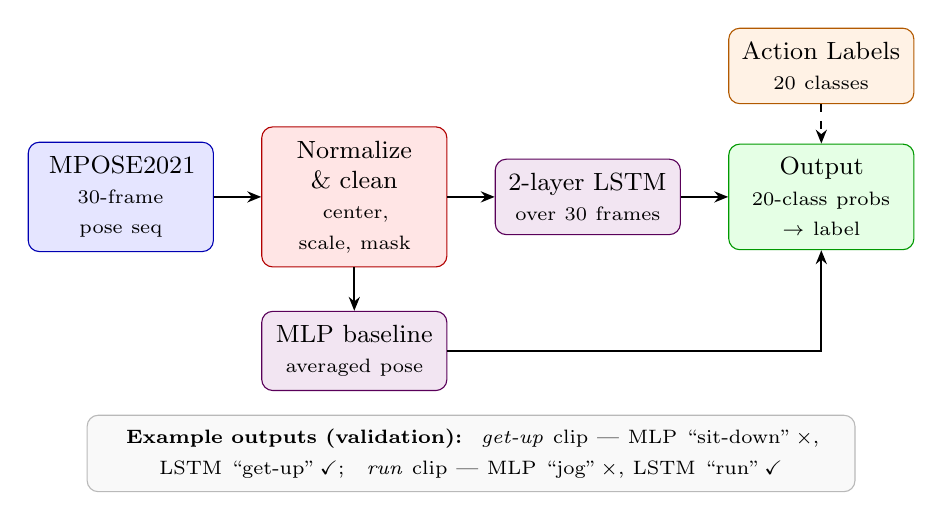
\begin{tikzpicture}[
  node distance=0.5cm and 0.6cm,
  box/.style={rectangle, rounded corners=4pt, align=center, font=\small,
              minimum height=0.9cm, text width=2.0cm, inner sep=5pt},
  arr/.style={-{Stealth[length=5pt, width=4pt]}, thick}
]
\node[box, draw=blue!70!black,   fill=blue!10]     (mpose)
  {MPOSE2021\\\scriptsize 30-frame pose seq};
\node[box, draw=red!70!black,    fill=red!10,      right=0.6cm of mpose] (prep)
  {Normalize \& clean\\\scriptsize center, scale, mask};
\node[box, draw=violet!70!black, fill=violet!10,   right=0.6cm of prep] (rnn)
  {2-layer LSTM\\\scriptsize over 30 frames};
\node[box, draw=green!60!black,  fill=green!10,    right=0.6cm of rnn] (eval)
  {Output\\\scriptsize 20-class probs $\to$ label};
\node[box, draw=violet!70!black, fill=violet!10,   below=0.55cm of prep] (mlp)
  {MLP baseline\\\scriptsize averaged pose};
\node[box, draw=orange!70!black, fill=orange!10,   above=0.5cm of eval] (labels)
  {Action Labels\\\scriptsize 20 classes};
\draw[arr] (mpose) -- (prep);
\draw[arr] (prep)  -- (rnn);
\draw[arr] (rnn)   -- (eval);
\draw[arr] (prep)  -- (mlp);
\draw[arr] (mlp.east) -| (eval.south);
\draw[arr, dashed] (labels) -- (eval);
\coordinate (cx) at ($(mpose)!0.5!(eval)$);
\node[box, draw=gray!55, fill=gray!5, text width=9.4cm, anchor=north] (ex)
  at ([yshift=-0.3cm]cx |- mlp.south)
  {\scriptsize\textbf{Example outputs (validation):}\;
   \emph{get-up} clip --- MLP ``sit-down''\,$\times$, LSTM ``get-up''\,$\checkmark$;\quad
   \emph{run} clip --- MLP ``jog''\,$\times$, LSTM ``run''\,$\checkmark$};
\end{tikzpicture}
\caption{System overview. \textbf{Input:} a 30-frame sequence of 17 body keypoints $(x,y,\mathrm{conf})$, normalised and cleaned. \textbf{Output:} a probability distribution over the 20 action classes; the highest-probability class is the predicted label. At deployment, frozen MoveNet supplies keypoints from webcam frames.}
\label{fig:pipeline}
\end{figure}

\section*{Background \& Related Work}
\textbf{BlazePose} \citep{bazarevsky2020blazepose} showed lightweight pose estimation runs in real time on-device and \textbf{HRNet} \citep{sun2019hrnet} demonstrated high-accuracy keypoint localisation, together motivating a frozen MoveNet-style front-end. \textbf{Hierarchical RNN} \citep{du2015hierarchical} established that recurrent networks recognise actions directly from skeleton sequences --- the approach adopted here. \textbf{ST-GCN} \citep{yan2018stgcn} instead treats the skeleton as a spatial-temporal graph, the canonical deep approach, though its gains rely on far larger datasets. \textbf{Action Transformer} \citep{mazzia2021action} released MPOSE2021 and reaches $\approx$0.9 accuracy with a substantially larger self-attention model.

\section*{Data Processing}
\textbf{Source and statistics.} MPOSE2021 \citep{mazzia2021action,mpose2021zenodo,pic4ser2021mpose} provides 30-frame clips of 17 COCO keypoints, shape \texttt{(30,17,3)} as $(x,y,\mathrm{conf})$, each labelled over 20 action classes and extracted with \emph{PoseNet} (see Architecture). The set has \textbf{15{,}429} clips and is heavily imbalanced: within the 12{,}562-clip official training split the largest class (\emph{walk}, 1{,}872) outnumbers the smallest (\emph{pick-up}, 197) by 9.5$\times$ (Figure~\ref{fig:data}).

\textbf{Cleaning and split (reproducible).} Each frame is (1)~\emph{normalised} --- centred at the mid-hip (mean of the two hip joints) and scaled by torso length (mid-hip to mid-shoulder distance, floored at $10^{-3}$ when those joints are themselves undetected) --- removing body size and screen position, as raw coordinates are pixels; (2)~\emph{cleaned} --- joints with confidence $<0.2$ have $(x,y,\mathrm{conf})$ zeroed \emph{after} normalisation, so a masked joint rests at the hip origin and is identified by its zero confidence channel; (3)~\emph{flattened} to per-frame 51-vectors, giving \texttt{(N,30,51)}. Inverse-frequency class weights $w_c = N/(K\,n_c)$ (0.34--3.19) feed a weighted cross-entropy loss, with macro-F1 as the headline metric. All results use official cross-subject \textbf{split~1}, whose test set was held out and scored once; validation was carved from train by stratified sampling (train 10{,}351 / val 2{,}211 / test 2{,}867).

\begin{figure}[!h]
\centering
\sbox0{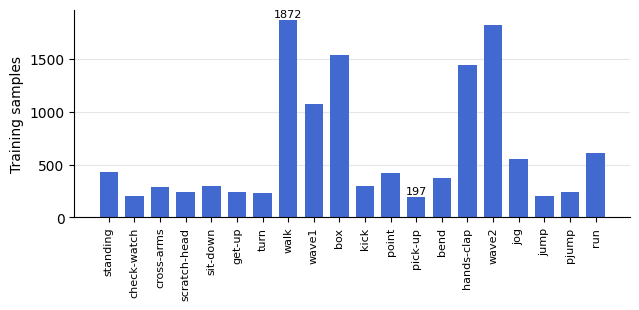
\includegraphics[width=0.36\linewidth]{class_distribution.png}}%
\usebox0\hfill
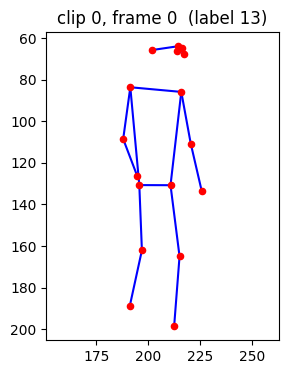
\includegraphics[height=\ht0]{cleaned_sample.png}
\caption{Left: class distribution over the 12{,}562-clip official training split (9.5$\times$ imbalance). Right: an example training frame's 17 keypoints plotted as a skeleton (raw pixel coordinates, before normalisation).}
\label{fig:data}
\end{figure}

\section*{Architecture}
The system has two stages. \textbf{Stage 1} supplies 17 COCO keypoints per frame and is never trained. MPOSE's precomputed PoseNet detections are used for all training and test-split results below, whereas deployment uses frozen MoveNet Thunder \citep{tensorflowmovenet}. Both output 17 COCO-format joints, so no remapping is needed; however, they remain different estimators. \textbf{Stage 2} is a \textbf{two-layer LSTM} (input 51, hidden 128 per layer, \texttt{batch\_first}, dropout 0.3 between layers); the top layer's final hidden state --- a summary of the whole motion --- passes through Dropout$(0.3)$ and \texttt{Linear(128,20)} to give class logits ($\approx$227K parameters). This many-to-one design uses LSTM gates over a plain RNN to retain information across all 30 frames. \textbf{Reproducibility:} seed 66, batch 64/256 (train/eval), Adam (lr $10^{-3}$), weighted cross-entropy, early stopping on validation macro-F1 (patience 15, 100-epoch cap; halted at 82, best weights from 67).

\section*{Baseline Model}
A \textbf{majority-class predictor} gives a trivial lower bound. The reported baseline is an \textbf{averaged-pose MLP}: the 30 frames are averaged into one 51-dim vector, classified by \texttt{Linear(51,128)} $\to$ ReLU $\to$ Dropout$(0.5)$ $\to$ \texttt{Linear(128,64)} $\to$ ReLU $\to$ Dropout$(0.5)$ $\to$ \texttt{Linear(64,20)} ($\approx$16K parameters), trained identically. Seeing the \emph{same} input but no temporal information, it isolates the value of temporal dynamics.

\section*{Quantitative Results}
\begin{table}[!h]
\centering\small
\begin{tabular}{lcccc}
\toprule
Model & Val acc & Val macro-F1 & Test acc & Test macro-F1 \\
\midrule
Majority-class (lower bound) & 0.15 & 0.01 & --- & --- \\
Averaged-pose MLP (baseline) & 0.63 & 0.56 & --- & --- \\
2-layer LSTM (primary)       & 0.87 & 0.82 & \textbf{0.82} & \textbf{0.75} \\
\bottomrule
\end{tabular}
\caption{In-distribution performance. On validation the MLP lifts macro-F1 from $\approx$0.01 to 0.56 and the LSTM to 0.82, a $+0.26$ margin attributable to temporal modelling. The test split --- scored once and reserved for the final model --- gives 0.82 accuracy and 0.75 macro-F1; the drop from validation reflects subject-independence, since validation subjects overlap training but test subjects do not.}
\label{tab:results}
\end{table}

Tuning was systematic: one change at a time, adopted only if the gain exceeded the measured $\pm$0.02 run-to-run noise. Seven variants --- regularisation, capacity, bidirectionality, pooling readouts, velocity features, their combination, augmentation --- fell within noise; one apparent winner (0.844) did not survive reseeding (0.827\,$\pm$\,0.015 over three seeds), leaving $\approx$0.82 macro-F1 as the best result across all tested configurations.

\section*{Qualitative Results}
The confusion matrices (Figure~\ref{fig:qual}) show \emph{why} the temporal model wins: the baseline's dominant errors are actions whose \emph{time-averaged} pose is nearly identical but whose \emph{motion} differs --- \textbf{get-up}/\textbf{sit-down} (0.64) and \textbf{run}/\textbf{jog} (0.41) --- which the LSTM collapses to 0.21 and 0.11. Its remaining errors ($\le$0.21) fall on ambiguous pairs: \textbf{point}$\,\to\,$\textbf{wave1} (0.18, similar single-arm trajectories) and \textbf{jump}$\,\to\,$\textbf{pjump} (0.11), separated only by global displacement (see Discussion).

\begin{figure}[!h]
\centering
\sbox0{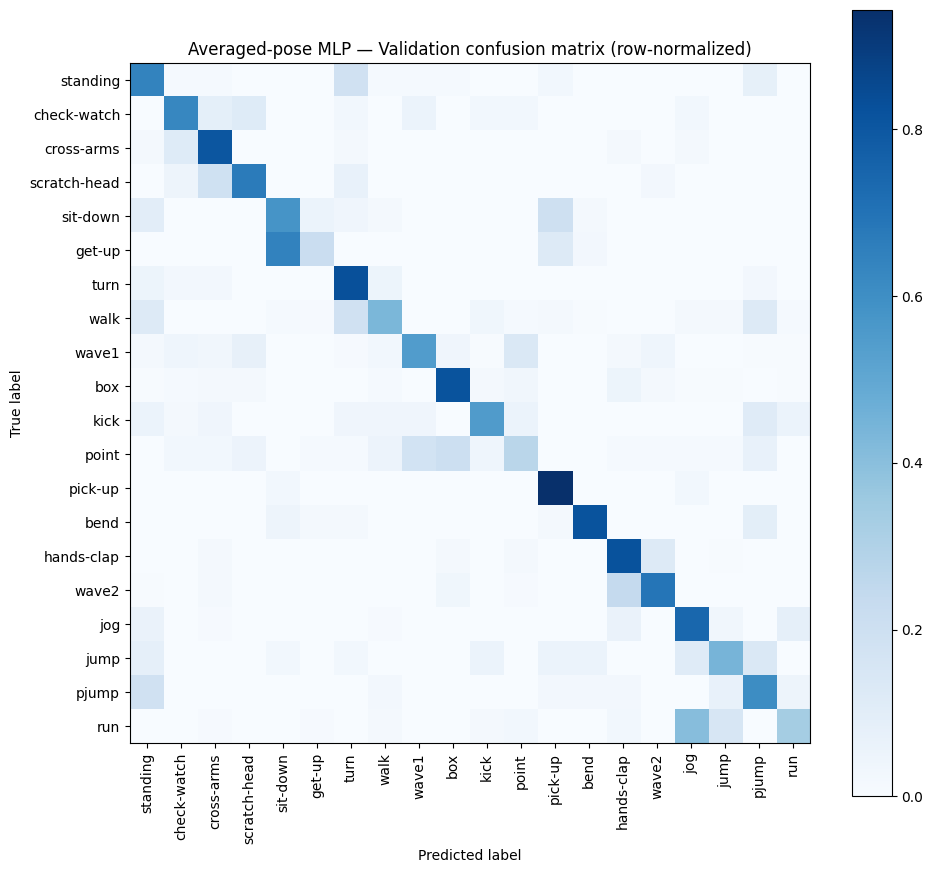
\includegraphics[width=0.37\linewidth]{mlp_confusion.png}}%
\usebox0\hfill
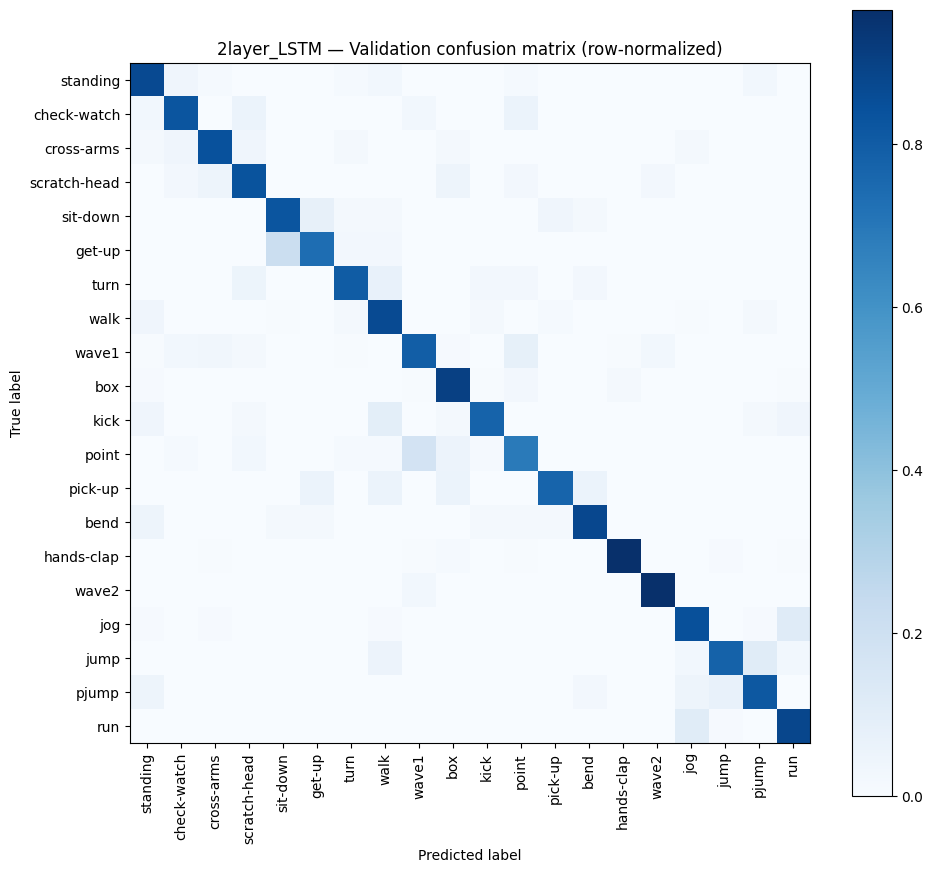
\includegraphics[height=\ht0]{rnn_confusion.png}
\caption{Row-normalised validation confusion matrices. Left: averaged-pose MLP baseline. Right: two-layer LSTM --- the motion-dependent confusions (get-up/sit-down, run/jog) are largely resolved.}
\label{fig:qual}
\end{figure}

\textbf{Sample outputs (from the self-recorded evaluation, below).} Examples were chosen to represent the dominant correct and incorrect patterns in the confusion matrices, not cherry-picked. Every \emph{sit-down} and \emph{bend} take was classified correctly, while a \emph{hands-clap} clip was read as \emph{cross-arms} (0.85; \emph{hands-clap} 0.15): with noisy wrists, hands meeting at the chest resemble crossed arms.

\section*{Evaluation on New Data}
\textbf{Tier 1: the official MPOSE cross-subject test split} (2{,}867 clips whose subjects never appear in training) was held out untouched throughout the project and scored exactly once, after tuning concluded: \textbf{0.82} accuracy / \textbf{0.75} macro-F1 (Table~\ref{tab:results}).

\textbf{Tier 2: self-recorded clips.} A fully out-of-distribution set was recorded with a MacBook webcam: \textbf{82} clips covering \textbf{18} of the 20 actions (up to 5 takes each). \emph{jog} and \emph{pick-up} were excluded: MPOSE ships skeletons, not source video, so their intended execution could not be inferred --- self-recorded versions would be meaningless test cases. To probe generalisation the clips were varied --- \textbf{four} locations (different backgrounds and lighting), \textbf{three} people of differing body proportions, varied position and speed --- with conditions fixed \emph{before} evaluation: static camera, full body in frame, one action per clip ($\approx$2--3\,s). Keypoints come from frozen MoveNet Thunder on a centre square crop, sampled as a centred 30-frame window at $\approx$30\,fps to match MPOSE's temporal resolution, then the \emph{identical} preprocessing. The clips never influenced training or tuning.

\textbf{Results.} The two-layer LSTM achieves \textbf{0.43} accuracy and \textbf{0.36} macro-F1 on the self-recorded set (Figure~\ref{fig:newdata}), versus 0.82/0.75 on the MPOSE test split; uniform guessing over the model's 20 outputs would score 0.05. The failures are systematic: large whole-body posture changes transfer well (\emph{sit-down}, \emph{bend}, \emph{cross-arms} 5/5; \emph{get-up}, \emph{walk}, \emph{run} 3/5), while low-motion classes (\emph{standing}, \emph{check-watch} 0/5) and fine arm gestures (\emph{hands-clap}, \emph{box}, \emph{kick} 1/5) collapse. With at most five takes per action these per-class rates indicate direction rather than magnitude. The temporal advantage persists: the MLP baseline reaches only 0.21 accuracy / 0.15 macro-F1 on the same clips. Given the compound shift, a substantial drop is the expected outcome; the informative result is its \emph{structure}.

\begin{figure}[!h]
\centering
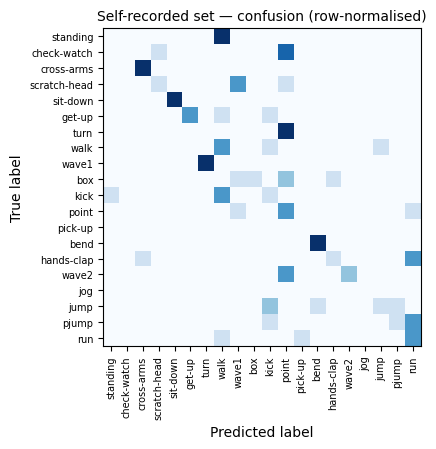
\includegraphics[width=0.40\linewidth]{new_data_confusion.png}
\caption{Row-normalised confusion on the self-recorded webcam set (82 clips, 18 actions).}
\label{fig:newdata}
\end{figure}

\section*{Discussion}
\textbf{Model capacity does not appear to be the primary bottleneck.} The most robust finding is negative. Seven systematic variants across architecture, readout, and input features remained within the run-to-run noise around 0.82 macro-F1. An apparent 0.844 breakthrough was exposed as a lucky seed by re-running under multiple seeds --- a reminder that in noisy training regimes, a compelling single result is not evidence. Strictly this establishes that capacity is not \emph{under}-provisioned rather than that data is the binding constraint; with $\approx$10K clips, graded class pairs and noisy keypoints the latter remains the more likely limit, and a learning curve over training-set size would test it directly.

\textbf{Where the error lives --- in and out of distribution.} The remaining confusions are largely structural. Hip-centring removes global displacement, making \emph{jump} and \emph{pjump} hard to separate: normalisation improves viewpoint invariance but discards information for classes defined by global motion. Separately, \emph{run} and \emph{jog} differ mainly in speed, a continuous rather than categorical boundary. Out of distribution, accuracy falls to 0.43 against 0.82 on the MPOSE test split for two plausible but, in this design, confounded reasons: a \emph{performance-style gap} --- the model learned MPOSE actors' renditions, and with no source video to imitate, the recorders' execution only approximates that style --- and an \emph{input-quality gap} --- the low-quality webcam yields keypoints averaging $\approx$0.61 confidence versus 0.81 in training, some joints missing outright, wrists least reliable. Large posture trajectories survive this noise; subtle gestures and no-motion classes are more easily obscured, so validation ranking did not predict deployment robustness. A surprising negative result: the augmentation-trained variant was expected to transfer \emph{better}, since the self-recorded clips contain exactly what its training noise simulated --- jittered coordinates and missing joints --- yet it scored \emph{lower} (0.35 vs.\ 0.43 accuracy); flip-and-jitter augmentation evidently does not capture the real shift's structure. Re-extracting the same clips with PoseNet would disentangle the two gaps --- holding subjects and style fixed while changing only the estimator --- and remains, with rotation normalisation and noise-calibrated augmentation, future work.

\textbf{What was learned.} The most striking lesson is how \emph{motion-sensitive} the recurrent model is: once video is reduced to joint coordinates, even tiny movements become prominent input signal. This likely explains the \emph{standing}$\,\to\,$\emph{turn} failure (a pilot \emph{standing} clip scored 0.76 for \emph{turn}): the recorded subjects were never perfectly still, and what a human observer dismisses as standing reads, in coordinate space, as deliberate motion.

\textbf{Scope.} The athletic framing is only partly supported: MPOSE2021's vocabulary is everyday activity, not sport technique, and the Tier-2 pattern --- coarse posture changes survive, fine limb gestures do not --- suggests the discrimination athletic feedback needs is what this pipeline loses first. Sport-specific analysis would require sport-specific data and a higher-fidelity extractor.

\textbf{Project difficulty.} The task is harder than its surface suggests: 20-way \emph{cross-subject} classification (no actor shared between train and test) from pose alone --- 51 numbers per frame, no appearance, object, or scene context --- on a modest corpus with 9.5$\times$ imbalance, noisy partially-missing keypoints, and class pairs (\emph{run}/\emph{jog}) that differ along a continuous rather than categorical boundary. Within those constraints the two-layer LSTM reaches 0.82 accuracy / 0.75 macro-F1 on cross-subject split~1 --- the accuracy is $\approx16\times$ the 0.05 chance level, and within reach of the $\approx$0.9 reported for the substantially larger Action Transformer released alongside the dataset \citep{mazzia2021action}. The work that most exceeds lab level is the evaluation itself: a protocol fixed before measurement, a measured noise floor with multi-seed verification of every candidate, and a self-built collection pipeline --- new subjects, locations, and pose estimator --- testing the model on data no part of the project had seen.


\section*{Ethical Considerations}
MPOSE2021 derives from human video, so licensing was confirmed for academic use. Its actors may not represent all body types, ages, or ethnicities, so accuracy may be uneven across users --- and a three-subject evaluation set is far too small to detect such unevenness. Because predicted labels could drive training feedback, misclassification could mislead an athlete: the system is a movement-analysis aid, not an authoritative judgement. Pose tracking can also become surveillance, so any deployment must obtain informed consent; the pose-only design (no raw video retained) is a deliberate privacy mitigation.

\newpage
\begin{thebibliography}{9}

\bibitem[Anthropic(n.d.a)]{anthropic2026claude}
Anthropic. (n.d.).
\newblock Claude.ai.
\newblock \url{https://claude.ai}. Accessed June 2, 2026.

\bibitem[Anthropic(n.d.b)]{anthropic2026claudecode}
Anthropic. (n.d.).
\newblock Claude Code.
\newblock \url{https://www.anthropic.com/claude-code}. Accessed June 2, 2026.

\bibitem[Bazarevsky et~al.(2020)]{bazarevsky2020blazepose}
Bazarevsky, V., Grishchenko, I., Raveendran, K., Zhu, T., Zhang, F., and Grundmann, M. (2020).
\newblock BlazePose: On-device real-time body pose tracking.
\newblock \textit{arXiv preprint arXiv:2006.10204}.

\bibitem[Du et~al.(2015)]{du2015hierarchical}
Du, Y., Wang, W., and Wang, L. (2015).
\newblock Hierarchical recurrent neural network for skeleton based action recognition.
\newblock \textit{CVPR}, 1110--1118.

\bibitem[Mazzia et~al.(2021)]{mazzia2021action}
Mazzia, V., Angarano, S., Salvetti, F., Angelini, F., and Chiaberge, M. (2021).
\newblock Action Transformer: A self-attention model for short-time pose-based human action recognition.
\newblock \textit{Pattern Recognition}, 124, 108487.

\bibitem[Mazzia et~al.(2021)]{mpose2021zenodo}
Mazzia, V., Angarano, S., Salvetti, F., Angelini, F., and Chiaberge, M. (2021).
\newblock MPOSE2021: A dataset for short-time pose-based human action recognition.
\newblock Zenodo. \url{https://zenodo.org/records/5803076}.

\bibitem[PIC4SeR(2021)]{pic4ser2021mpose}
PIC4SeR. (2021).
\newblock MPOSE2021\_Dataset.
\newblock \url{https://github.com/PIC4SeR/MPOSE2021_Dataset}.

\bibitem[Sun et~al.(2019)]{sun2019hrnet}
Sun, K., Xiao, B., Liu, D., and Wang, J. (2019).
\newblock Deep high-resolution representation learning for human pose estimation.
\newblock \textit{CVPR}, 5693--5703.

\bibitem[TensorFlow Hub(2024)]{tensorflowmovenet}
TensorFlow Hub. (2024).
\newblock MoveNet: Ultra fast and accurate pose detection model.
\newblock \url{https://www.tensorflow.org/hub/tutorials/movenet}.

\bibitem[Yan et~al.(2018)]{yan2018stgcn}
Yan, S., Xiong, Y., and Lin, D. (2018).
\newblock Spatial temporal graph convolutional networks for skeleton-based action recognition.
\newblock \textit{AAAI Conference on Artificial Intelligence}, 7444--7452.

\end{thebibliography}

\end{document}
